\subsection{Analog-To-Digital Converter:}

Once the Circuit of Figure 3.0 were assembled, we connected the {\bfseries LM35} to the terminal 6 of the {\bfseries ADC0804}, then, with the help of a lighter we variate the temperature of the sensor, this provided different voltage levels. \hfill \break

{\bfseries\itshape\color{carmine}{Observation:}} {\itshape\color{carmine}{Both devices ( {\bfseries ADC0804} and {\bfseries LM35} ) must be connected to a 5 $V_{cc}$ source.}} \hfill \break

\begin{figure}[H]
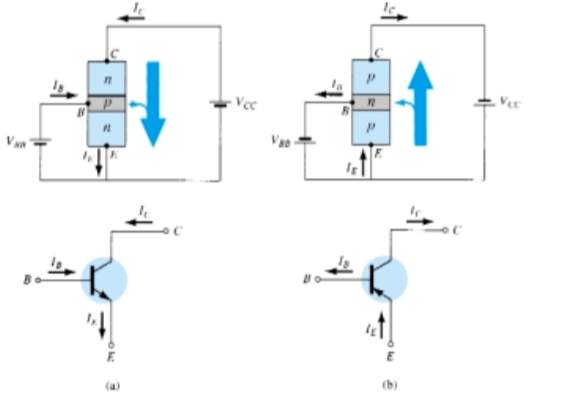
\includegraphics[height = 8cm, width = 16.5cm]{5.png}
\centering \linebreak \linebreak {\small Figure 3.0: Analog-to-digital converter circuit.}
\end{figure}

\begin{figure}[H]
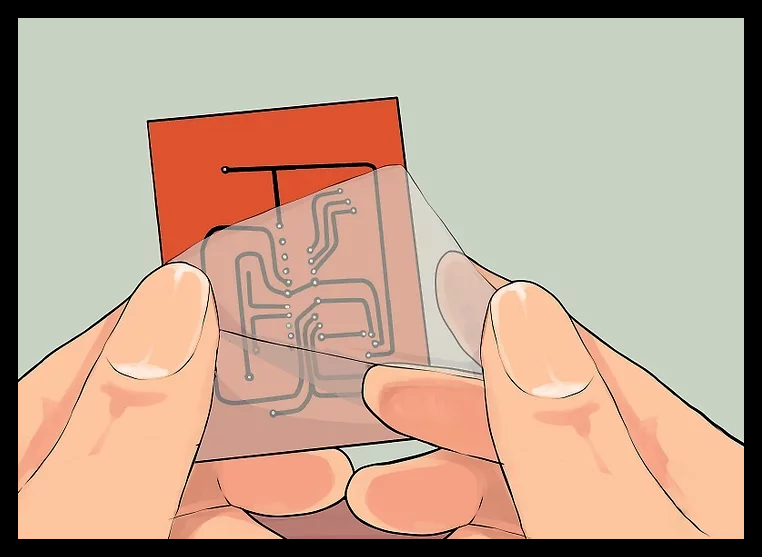
\includegraphics[height = 8cm, width = 16.5cm]{6.png}
\centering \linebreak \linebreak {\small Figure 3.1: {\bfseries LM35} diagram.}
\end{figure} \hfill \break

\pagebreak

Table 1 provide in its first column the voltage of the sensor, in its third column it's represented the binary-combination ( the terminal 18 of the {\bfseries ADC0804} it's the least-significant bit and the terminal 11 it's the most-significant bit ) that the {\bfseries ADC} provided on its output and the second column it's the temperature of the sensor. This are the final results of the practice that later will be compared with the {\itshape Theoretical} and {\itshape Simulated} results. \hfill \break

\begin{center}
\begin{tabular}{c c c c}
\toprule \toprule
\hspace{40px} Sensor Voltage \hspace{40px} & \hspace{30px} Temperature \hspace{30px} & \hspace{30px} Binary Combination \hspace{30px} \\
\midrule \midrule
0.42 V & $42^{\circ}$ & 0010 1011 & \\
\midrule
0.39 V & $39^{\circ}$ & 0010 1000 & \\
\midrule
0.36 V & $36^{\circ}$ & 0010 0101 & \\
\midrule
0.35 V & $35^{\circ}$ & 0010 0100 & \\
\midrule
0.33 V & $33^{\circ}$ & 0010 0010 & \\
\midrule
0.31 V & $31^{\circ}$ & 0010 0000 & \\
\midrule
0.29 V & $29^{\circ}$ & 0001 1110 & \\
\midrule
0.27 V & $27^{\circ}$ & 0001 1100 & \\
\bottomrule
\end{tabular}
\centering \linebreak \linebreak Table 1: Practice results.
\end{center}

\pagebreak